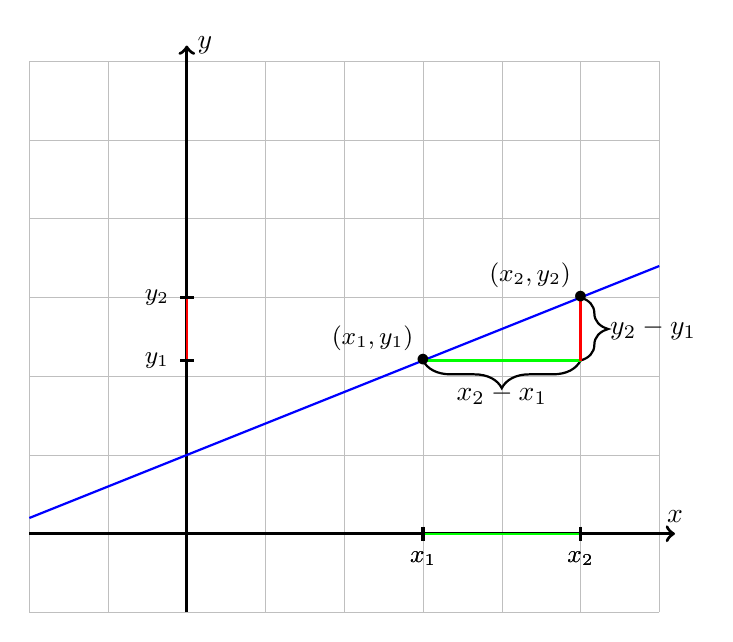
\begin{tikzpicture}
  \def\a{3}
  \def\b{2.2}
  \def\c{5}
  \def\d{3}
  \path [draw, help lines, opacity=.5]  (-2,-1) grid (6,6);

  \draw [very thick] (\a,2.5pt) -- +(0,-5pt) node [anchor=north, font=\small] {$x_1$}
	[very thick] (\c,2.5pt) -- +(0,-5pt) node [anchor=north, font=\small] {$x_2$};

	\draw [very thick,->] (-2,0) -- (6+.2,0) node [anchor=south] {$x$};
	\draw [very thick,->] (0,-1) -- (0,6+.2) node [anchor=west] {$y$};
	\draw [thick,green] (\a,0) -- (\c,0);
	\draw [thick,red] (0,\b) -- (0,\d);
	
	\draw [very thick] (\a,2.5pt) -- +(0,-5pt) node [anchor=north, font=\small] {$x_1$}
	      [very thick] (\c,2.5pt) -- +(0,-5pt) node [anchor=north, font=\small] {$x_2$}
	      (2.5pt,\b) -\- +(-5pt,0) node [anchor=east, font=\small] {$y_1$}
	      (2.5pt,\d) -\- +(-5pt,0) node [anchor=east, font=\small] {$y_2$};

	      \draw [thick, blue] (-2,0.2) -- (6,3.4);
	      \node [above left] at (\a, \b) [font=\small] {$(x_1, y_1)$};
	      \node [above left] at (\c,\d) [font=\small] {$(x_2, y_2)$};

	      \draw[thick,decorate,decoration={brace,amplitude=10pt,mirror}] (\a,\b) -- (\c,\b) node [midway,below,yshift=-5pt] {$x_2 - x_1$};
	      \draw [thick,green] (\a,\b) -- (\c,\b);


	      \draw[thick,decorate,decoration={brace,amplitude=10pt,mirror}] (\c,\b) -- (\c,\d) node [midway,right,xshift=7pt] {$y_2 - y_1$};
	      \draw [thick,red] (\c,\b) -- (\c,\d);
	      
	      \node at (\a, \b) {$\bullet$};
	      \node at (\c, \d) {$\bullet$};
	      
\end{tikzpicture}
